\documentclass[final]{beamer}

\usepackage[T1]{fontenc}
\usepackage{lmodern}
\usepackage[orientation=portrait,size=a1,scale=1.1]{beamerposter}
\usetheme{gemini}
\usecolortheme{mit}
\usepackage{amsmath}
\usepackage{amssymb}
\usepackage{amsfonts}
\usepackage{dsfont}
\usepackage{xcolor}
\usepackage{pgfplots}
\pgfplotsset{compat=1.18}
\usepackage{graphicx}
\usepackage{array}
\usepackage{booktabs}
\usepackage{hyperref}
\usepackage{anyfontsize}
\usepackage[absolute,overlay]{textpos}

\newlength{\sepwidth}
\newlength{\colwidth}
\setlength{\sepwidth}{0.03333\paperwidth}
\setlength{\colwidth}{0.45\paperwidth}

\newcommand{\separatorcolumn}{\begin{column}{\sepwidth}\end{column}}

\title{Adaptive Graph Transform Clustering via Rate-Distortion Optimization for Point Cloud Attribute Compression}

\author{Simón Yáñez \inst{1} \and Eduardo Pavez \inst{2} \and Jorge Silva \inst{1}}

\institute[shortinst]{{
  \inst{1} Departamento de Ingeniería Eléctrica, Universidad de Chile \\
  \inst{2} University of Southern California \\
  \textbf{EL7024 - Teoría de Información: Fundamentos y Aplicaciones}
}}

\footercontent{
  Sesión de Pósters - Teoría de Información: Fundamentos y Aplicaciones \hfill \href{mailto:simon.yanez@ug.uchile.cl}{simon.yanez@ug.uchile.cl}
}

\begin{document}

\begin{textblock*}{0.08\paperwidth}(0.03\paperwidth,0.04\paperheight)
  
\includegraphics[width=2\linewidth]{logos/FCFM.pdf}
\end{textblock*}

\begin{textblock*}{0.1\paperwidth}(0.855\paperwidth,0.055\paperheight)
  
\includegraphics[width=\linewidth]{logos/die.pdf}
\end{textblock*}

\begin{frame}[t]
\begin{columns}[t]
\separatorcolumn

\begin{column}{\colwidth}

\begin{block}{Introduction}
Point clouds (PC) are essential for 3D representation, but their unstructured nature and high density demand efficient compression. While geometry compression is well-studied, attribute (color/luminance) compression remains a challenge. We propose a framework that adapts the \textbf{Graph Fourier Transform (GFT)} to local signal trends through \textbf{RD-Optimized Clustering}, creating a dictionary of transforms that compacts energy better than static geometry-based graphs.
\end{block}

\begin{block}{Innovation 1: Adaptive Graph Topology}
Standard GFT uses a \textbf{Structural Graph} ($\mathcal{G}_s$) where weights $W_{ij}$ depend only on spatial distance. We introduce the \textbf{Attribute Graph} ($\mathcal{G}_a$), which modifies $\mathcal{G}_s$ by adding \textbf{self-loops} to nodes that act as "sinks" in the attribute gradient field.

\vspace{0.5em}
\textbf{Mathematical Formulation:}
\begin{enumerate}
    \item \textbf{Attribute Motion:} $M_{ij} = W_{ij} \cdot (y_i - y_j)$ where $y$ is the luminance.
    \item \textbf{Sink Identification:} Nodes $j$ with the highest incoming gradient count $S_j$ are selected.
    \item \textbf{Topology Adaptation:} $W_{jj} = w_{sl}$ for the top $\tau\%$ of sink nodes.
\end{enumerate}
This forces the GFT basis vectors to align with the local signal trend, maximizing energy compaction.
\end{block}

\begin{block}{Innovation 2: RD-Optimized Clustering}
We learn a codebook of $K$ transforms (defined by slopes $\vec{s}_k$ and self-loop parameters). Unlike K-means, assignments are based on the \textbf{Lagrangian Cost} $J = D + \lambda R$.

\vspace{0.5em}
\textbf{The Training Loop:}
\begin{itemize}
    \item \textbf{Assignment (Expectation):} Blocks choose the transform minimizing $J$. \textbf{Simulated Annealing} is used to explore the cost surface and avoid local minima.
    \item \textbf{Optimization (Maximization):} Transform parameters ($\vec{s}, w_{sl}, \tau$) are refined using \textbf{Differential Evolution} to minimize the total RD-cost of the assigned blocks.
\end{itemize}
\end{block}

\begin{block}{Innovation 3: Spatial Regularization \& Dilution}
A major contribution of this work is identifying and solving the \textbf{Signaling Tax} problem. Even if an adaptive transform is superior, the cost of signaling the choice (cluster ID) can outweigh the gains.

\vspace{0.5em}
\textbf{Methodology:}
\begin{enumerate}
    \item \textbf{Viterbi-Style Smoothing:} We add a penalty $\beta$ for cluster-switching between Morton-adjacent blocks: $J_{total} = \sum (D_i + \lambda R_i) + \beta \cdot \mathds{1}(L_i \neq L_{i-1})$.
    \item \textbf{CABAC Signaling:} We use 1st-order conditional entropy $H(L_i | L_{i-1})$ to exploit the runs created by $\beta$.
    \item \textbf{Overhead Dilution:} By increasing block size ($B=16, 32$), the signaling overhead is spread over more points, making the "tax" negligible.
\end{enumerate}
\end{block}

\end{column}
\separatorcolumn

\begin{column}{\colwidth}

\begin{block}{The Scaling Frontier: RD Results}

\begin{figure}
\centering
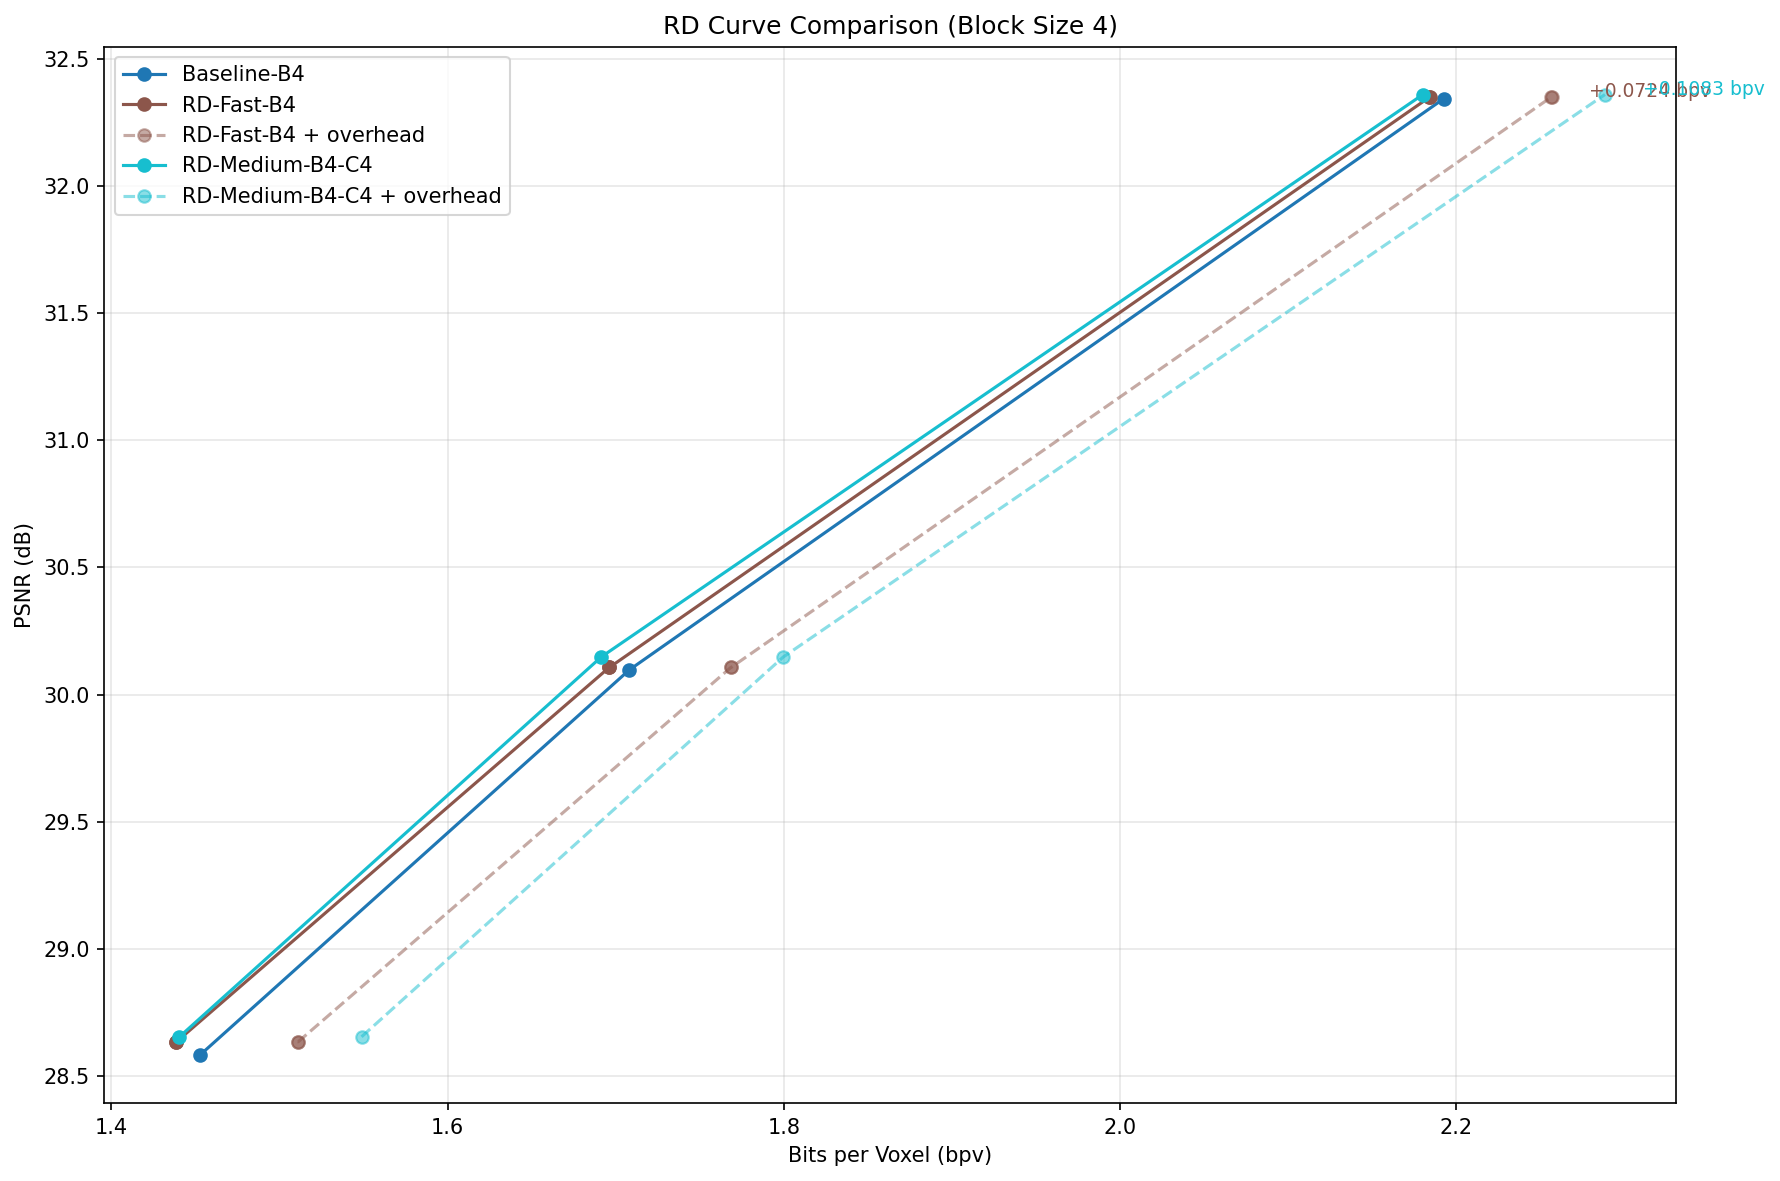
\includegraphics[width=0.45\linewidth]{B4_rd_comparison.png}
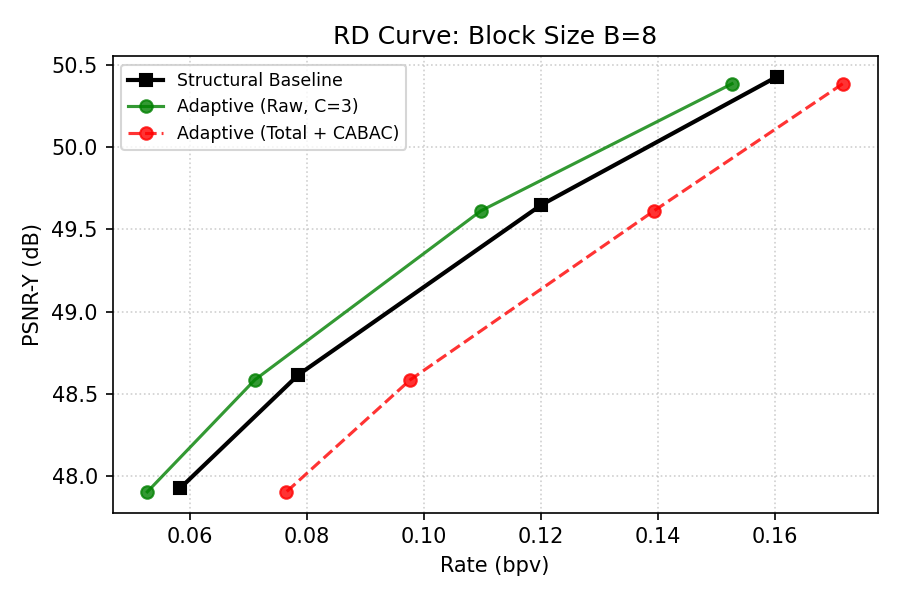
\includegraphics[width=0.45\linewidth]{B8_rd_comparison.png}\\[0.5em]
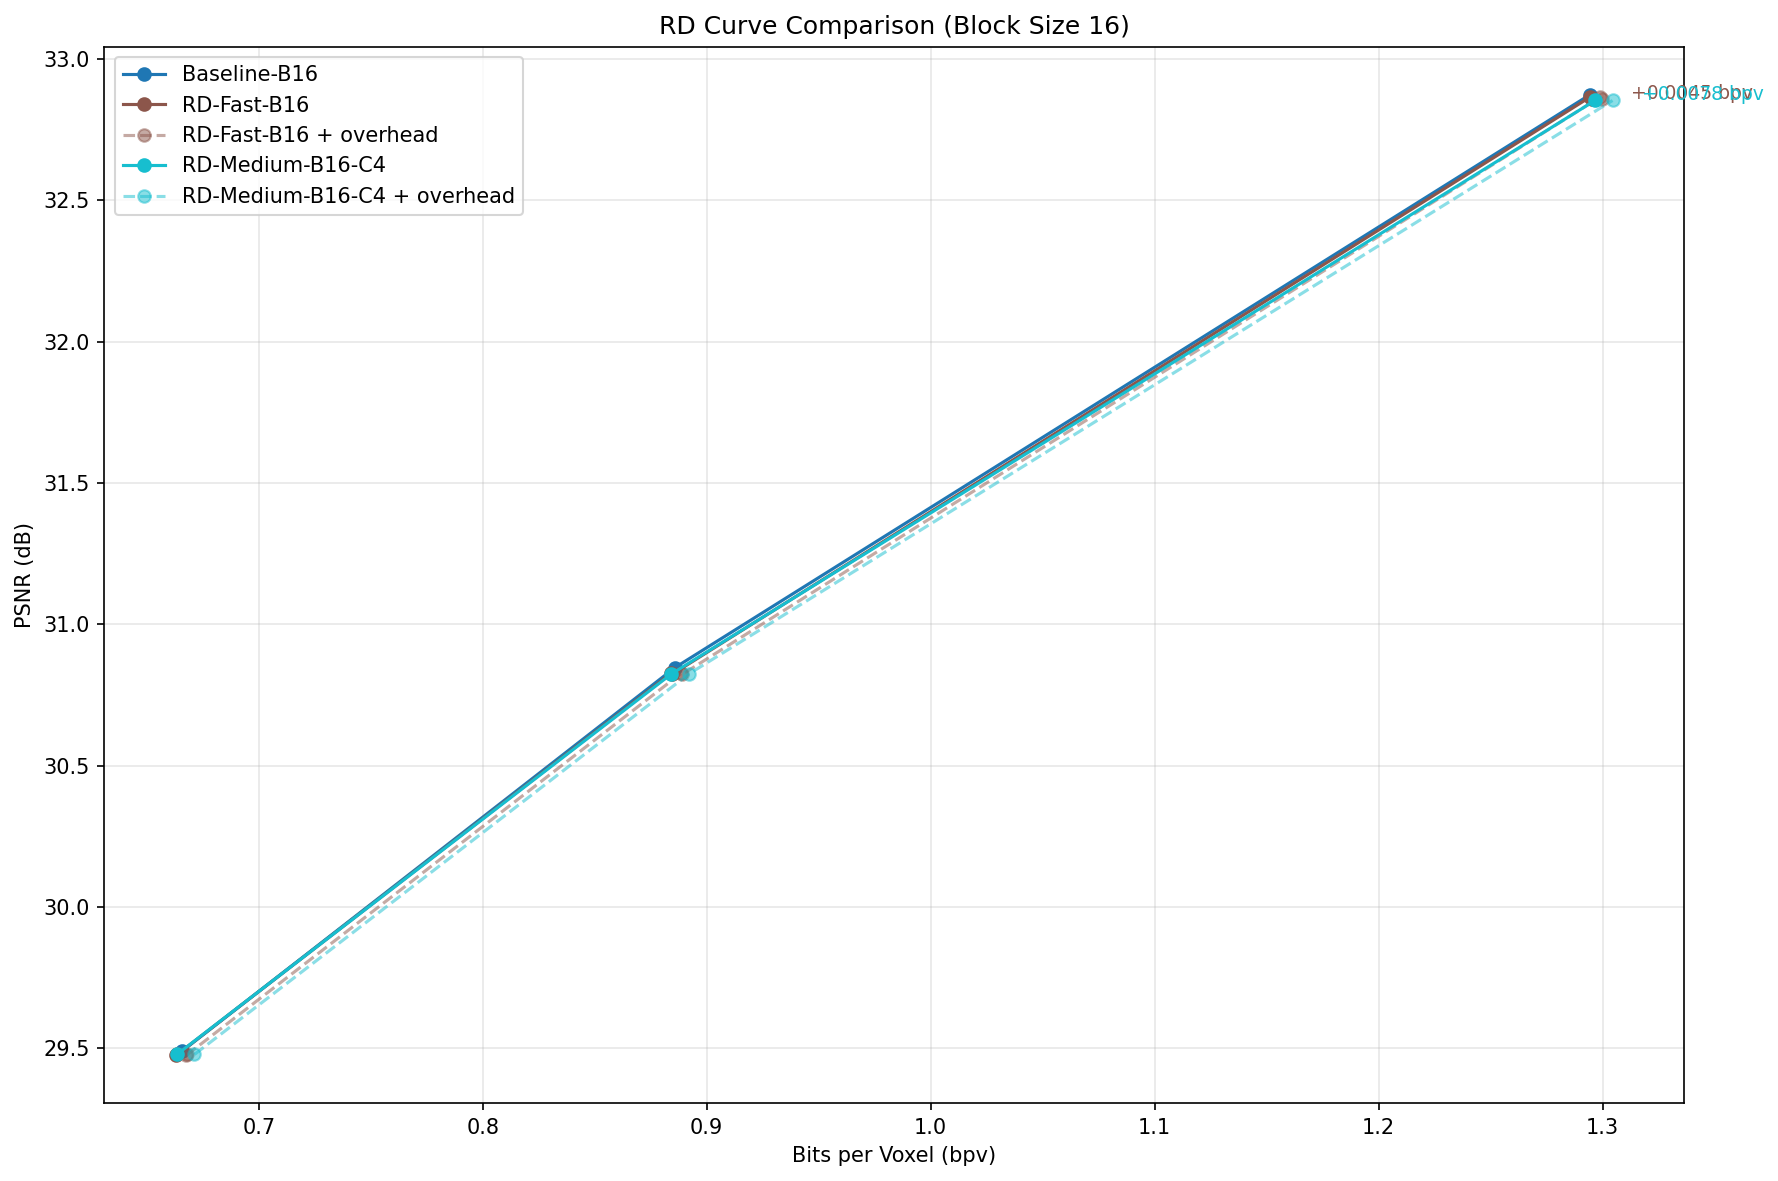
\includegraphics[width=0.45\linewidth]{B16_rd_comparison.png}
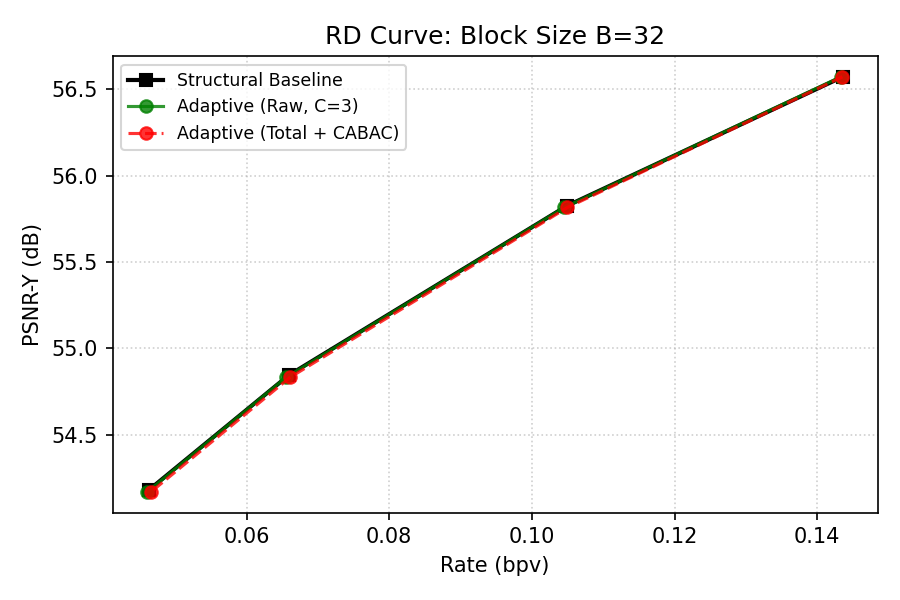
\includegraphics[width=0.45\linewidth]{B32_rd_comparison.png}
\caption{RD Curves (PSNR-Y vs bpv). Green: Transform Gain (Raw). Red Dotted: Total Rate (including CABAC overhead). Black: Structural Baseline.}
\end{figure}

\vspace{0.5em}
\textbf{Analysis of the Scale Effect:}
\begin{itemize}
    \item \textbf{B4/B8:} While these scales show the highest \textit{Raw Gains} (green line far from black), the \textit{Signaling Tax} (red line) is prohibitive.
    \item \textbf{B16:} The break-even point. Overhead drops to $\sim$0.004 bpv.
    \item \textbf{B32:} The \textbf{Compression Breakthrough}. Overhead is diluted to $<$0.001 bpv, allowing adaptive gains to yield a negative net gain.
\end{itemize}
\end{block}

\begin{block}{Performance Summary (Q=24)}
\begin{table}[h]
\centering
\small
\begin{tabular}{@{}lccc@{}}
\toprule
\textbf{Config ($K=4$)} & \textbf{Overhead (bpv)} & \textbf{Raw Saving} & \textbf{Net Gain} \\
\midrule
Small Detail (B4) & 0.0239 & -1.4\% & \textcolor{red}{+10.47\%} \\
Medium Scale (B8) & 0.0189 & -4.8\% & \textcolor{red}{+7.02\%} \\
Large Scale (B16) & 0.0042 & -2.2\% & \textcolor{gray}{+0.61\%} \\
\textbf{Global (B32)} & \textbf{0.0002} & \textbf{-0.2\%} & \textbf{\textcolor{blue}{-0.03\%}} \\
\bottomrule
\end{tabular}
\caption{Full Point Cloud results with CABAC overhead estimation.}
\end{table}

\vspace{0.5em}
\textbf{Key Insights:}
\begin{itemize}
    \item \textbf{Spatial Penalty ($\beta=2000$)} reduced CABAC overhead by \textbf{72\%} vs memoryless entropy.
    \item \textbf{Unit Discrepancy:} Training gains in $D$ (MSE) can be massive (25\%+) while bit-savings are small. High $\lambda \geq 5.0$ is required for compression-first dictionaries.
\end{itemize}
\end{block}

\begin{block}{Conclusions}
This work validates that \textbf{Attribute-Dependent Graph Transforms} can achieve true compression if the signaling overhead is managed through \textbf{spatial regularization} and \textbf{scale management}. 

We proved that B32 is the optimal production scale for per-block signaling, while B4/B8 are only suitable for high-fidelity scenarios where bit-rate is secondary to reconstruction quality. Future work will explore \textbf{skip-mode signaling} to further reduce the tax on structural blocks.
\end{block}

\begin{block}{References}
\footnotesize{\bibliographystyle{plain}\bibliography{poster}}
\end{block}

\end{column}
\separatorcolumn
\end{columns}
\end{frame}
\end{document}
